\chapter{Desenvolvimento e Implementação}
\label{ch::implement}

\section{Introdução}
\label{sec::implement:intro}

A fase de implementação, que se estendeu por cerca de 2 semanas, envolveu a execução paralela de diferentes tarefas pelos dois elementos do grupo. Este Capítulo aborda em particular os seguintes aspetos desta fase do projeto:

\begin{itemize}%[nosep]
	\item Escolhas de implementação (Secção \ref{sec::implement:escolhas}): explica as decisões feitas durante a implementação do código-fonte;
	\item Detalhes de implementação (Secção \ref{sec::implement:detalhes}): explora os detalhes mais importantes e/ou interessantes no código-fonte.
\end{itemize}

Adicionalmente, são descritos o manual de instalação (Secção \ref{sec::implement:instalar}) e %: aborda a compilação da aplicação e a respetiva instalação num \textit{smartphone} com sistema operativo \textit{Android}\texttrademark;
o manual de utilização (Secção \ref{sec::implement:utilizacao}). %: exemplifica o uso da aplicação final na ótica do utilizador.


\section{Escolhas de Implementação}
\label{sec::implement:escolhas}

A primeira e grande escolha de implementação que se faz notar ao longo de todo o código é a utilização de classes e das bibliotecas providenciadas pelo C++ a fim de tirar o máximo partido desta linguagem de programação.

Desta forma, o código-fonte está organizado nas seguintes pastas:

\begin{itemize}
    \item \verb|bin|: inclui o binário compilado e as seguintes pastas:
    \begin{itemize}[nosep]
        \item \verb|fonts|: localização das fontes utilizadas para renderizar texto;
        \item \verb|shaders|: alberga os \textit{fragment shaders} e os \textit{vertex shaders} para a renderização das moléculas e do texto.
    \end{itemize}
    \item \verb|deps|: pasta gerada pelo \textit{Makefile} para gerir as dependências durante a compilação;
    \item \verb|doc|: aloja a documentação do projeto (nomeadamente o presente relatório);
    \item \verb|include|: pasta com os \textit{header files} de todos os métodos e classes utilizados no projeto;
    \item \verb|obj|: pasta gerada pelo \textit{Makefile} para guardar os ficheiros objeto a serem compilados no executável final;
    \item \verb|src|: alberga todos os códigos-fonte (ficheiros \verb|*.cpp|) com a implementação dos métodos e das classes declaradas nos \textit{header files} da pasta \verb|include|.
\end{itemize}


\section{Detalhes de Implementação}
\label{sec::implement:detalhes}

O ficheiro principal, \verb|bohr.cpp|, aloja a função \verb|main()| de onde o programa arranca. Aqui são invocadas as seguintes funções de inicialização:

\begin{minted}[breaklines,linenos]{cpp}
GLFWwindow* initialize_glfw(int width, int height, const char* title);
int initialize_glad(void);
\end{minted}

Estas funções inicializam, respetivamente, as bibliotecas GLFW e GLAD, necessárias para a comunicação com a \ac{API} do \opengl. Caso a primeira função retorne \verb|NULL| ou a segunda retorne \verb|0|, é gerada uma mensagem de erro na linha de comandos e o programa é abortado. A função de inicialização do GLFW em particular associa as funções de \textit{callback} para o teclado e para o rato.

De seguida são compilados os \textit{shaders} de renderização das moléculas com recurso à classe \textit{Shader} (implementada em \verb|shader_m.cpp|):

\begin{minted}[breaklines,linenos]{cpp}
debug("Loading shaders...\n");
Shader lightingShader = Shader("shaders/lighting_vs.glsl", "shaders/lighting_fs.glsl");
\end{minted}

Esta classe fornece métodos rápidos e muito acessíveis para manipular os dados passados aos \textit{shaders} e a respetiva utilização.

É ainda inicializado o renderizador de texto:

\begin{minted}[breaklines,linenos]{cpp}
TextRenderer textrenderer = TextRenderer(SCR_WIDTH, SCR_HEIGHT);
try {
    textrenderer.Load("fonts/UbuntuMono-R.ttf", 24);
} catch (const std::exception &e) {
    std::cerr << e.what() << '\n';
}
\end{minted}

A classe \textit{TextRenderer} está disponível \textit{online} \cite{textrender} para livre utilização, assim como os \textit{shaders} para a renderização deste mesmo texto.

Por fim, o programa entra no seu ciclo de renderização. Este começa por limpar o \textit{buffer} atual e renderiza os textos, nomeadamente as instruções no canto superior esquerdo e o nome do ficheiro (se aberto) no canto inferior esquerdo.

De imediato é processado o \textit{input} de teclado do utilizador com a seguinte função:

\begin{minted}[breaklines,linenos]{cpp}
action processInput(GLFWwindow *window, char **fname);
\end{minted}

Esta função ajusta os parâmetros da câmara conforme as teclas selecionadas, mas em particular trata de abrir a janela de diálogo para abrir um ficheiro novo com o seguinte excerto de código:

\begin{minted}[breaklines,linenos]{cpp}
if (glfwGetKey(window, GLFW_KEY_O) == GLFW_PRESS) {
    switchModeView(window, false);
    if (*fname != NULL) free(*fname);
    *fname = openPDBFileDialog();
    switchModeView(window, true);
    return (*fname != NULL) ? action::OPEN_FILE : action::NO_ACTION;
}
\end{minted}

O modo de visualização é temporariamente alterado a fim de permitir que o cursor do rato seja visível durante a seleção do ficheiro uma vez que este é oculto durante a renderização da molécula. Após obter o caminho para o ficheiro pretendido, a função verifica se porventura não será \verb|NULL|: neste caso, a molécula renderizada atualmente mantém-se e não é apagada da memória. Caso contrário, é devolvido um enumerador do tipo \verb|action| que indica que o utilizador selecionou um novo ficheiro:

\begin{minted}[breaklines,linenos]{cpp}
typedef enum {
    NO_ACTION,
    CAMERA_RESET,
    OPEN_FILE
} action;
\end{minted}

No ciclo de renderização é feita uma análise deste retorno a fim de determinar a próxima ação. O \textit{reset} da câmara envolve a invocação da seguinte chamada:

\begin{minted}[breaklines,linenos]{cpp}
camera = molecule.resetCamera();
\end{minted}

Esta função será vista mais à frente.

Caso seja aberto um novo ficheiro, a sua extensão é verificada como forma de validação primária:

\begin{minted}[breaklines,linenos]{cpp}
bool isPBD(char *fname) {
    return
    string(std::experimental::filesystem::
        path(fname).extension())
        .compare(".pdb") == 0;
}
\end{minted}

Sendo um ficheiro \ac{PDB}, a seguinte linha de código irá carregar uma nova molécula a partir do ficheiro selecionado pelo utilizador:

\begin{minted}[breaklines,linenos]{cpp}
    molecule = Molecule().fromPDB(fname);
\end{minted}

Por fim, a molécula é renderizada de forma a apresentar a superfície de \textit{van der Walls}:

\begin{minted}[breaklines,linenos]{cpp}
molecule.render_vanderWalls(lightingShader, camera, screen_width, screen_height, molrotx, molroty);
\end{minted}

À classe \textit{Molecule}, implementada no ficheiro \verb|pdbreader.cpp|, são delegadas todas as seguintes tarefas:

\begin{itemize}
    \item Ler o ficheiro \ac{PDB} e fazer o respetivo \textit{parsing} a fim de obter os átomos e as respetivas coordenadas;
    
    \item Obter os dados relativos a cada átomo dada a tabela periódica implementada em \verb|ptable.h|, nomeadamente o raio de \textit{van der Walls} \cite{ptable} e a cor CPK \cite{cpk};
    
    \item Computar as esferas associadas a cada átomo dado o raio determinado anteriormente;
    
    \item Renderizar as esferas nas posições correspondentes às coordenadas do respetivo átomo e com a respetiva cor;
    
    \item Determinar a posição inicial da câmara dada a dimensão da molécula processada através do método \verb|resetCamera()|.
\end{itemize}

Após estudo do formato de ficheiros \ac{PDB}, determinou-se que o \textit{parsing} seria simplificado uma vez que as posições de cada dado é esperado exatamente sempre na mesma posição de cada linha, em particular:

\begin{itemize}
    \item Três coordenadas nas posições 30, 38 e 46 da linha;
    \item Símbolo atómico na posição 76.
\end{itemize}

Só as linhas começadas por \verb|ATOM| ou \verb|HETATM| são interpretadas uma vez que são estas aquelas que contêm os dados relativos aos átomos. Uma vez que só é pretendida a superfície, não é necessário calcular as ligações entre átomos (o formato \ac{PDB} não fornece esta informação explicitamente).

Dada a política determinada anteriormente na Secção \ref{sec::implement:escolhas}, a classe \textit{Molecule} \textbf{não} é responsável por calcular os pontos das esferas. Uma classe própria existe para o efeito, \textit{VBOSphere}, sendo então criadas instâncias desta classe num vetor:

\begin{minted}[breaklines,linenos]{cpp}
bool Molecule::generateSpheres(void) {
    this->spheres = vector<VBOSphere>();
    for (auto atom : this->atoms) {
        this->spheres.push_back(VBOSphere(atom.radius, 50, 50, PeriodicTable::getColorFromSymbol(atom.name)
            .toVec3()));
    }
    return true;
}
\end{minted}

Classes e estruturas (\textit{structs}) foram criadas para lidar com pontos e cores a fim de fornecer métodos imediatos para os converter no tipo de dados \verb|glm::vec3| através da função \verb|toVec3()|, comum a ambas as classes.

A renderização da molécula passa por um ciclo que percorre todas as esferas anteriormente computadas, carregando no respetivo \textit{shader} a cor de cada esfera e a posição da câmara como fonte de luz. É de igual forma feita a transformação no mundo através de rotação, translação e escala (exatamente por esta ordem) a fim de posicionar a esfera no local exato. Bastará nesta fase invocar o seguinte método:

\begin{minted}[breaklines,linenos]{cpp}
this->spheres[i].render();
\end{minted}

O resultado final é semelhante ao do exemplo da Figura \ref{fig::bohr-main}.


\section{Manual de Instalação}
\label{sec::implement:instalar}

O projeto foi implementado primariamente para o sistema operativo \textit{Linux}. Em especial, foi utilizado o \textbf{\textit{Linux Mint} 20.0} com as mais recentes atualizações em dia.

A fim de compilar o projeto, é necessário ter as seguintes bibliotecas instaladas no sistema:

\begin{itemize}[nosep]
    \item \verb|g++|;
    \item \verb|make|;
    \item \verb|libglfw3-dev|;
    \item \verb|libglm-dev|;
    \item \verb|freetype|.
\end{itemize}

O \textit{Makefile} incluído tratará da compilação de todos os ficheiros de forma automática, sendo fornecidos três modos:

\begin{enumerate}
    \item \verb|make debug|: compila no modo \textit{debug}, o qual providencia informações adicionais durante a execução para fins de desenvolvimento;
    \item \verb|make release|: compila no modo \textit{release}, ou seja, cria uma versão final para o utilizador final;
    \item \verb|make clean|: elimina todas as dependências, ficheiros objeto e executáveis a fim de se poder realizar uma compilação fresca de seguida.
\end{enumerate}


\section{Manual de Utilização}
\label{sec::implement:utilizacao}

Com o projeto compilado, é \textbf{peremptória} a execução do programa através da linha de comandos \textbf{dentro da pasta} onde se encontra o executável. A sua execução é alcançada da seguinte forma:

\begin{verbatim}
./bohr
\end{verbatim}

Ao abrir, a aplicação apresenta apenas as opções disponíveis e indica no fundo a informação ``\textit{No file opened}'' (Figura \ref{fig::bohr-start}). As opções são as seguintes:

\begin{itemize}[nosep]
    \item Tecla \verb|O|: abrir ficheiro \ac{PDB};
    \item Teclas \verb|WASD|: mover a câmara;
    \item Rato: rodar a câmara;
    \item Teclas \verb|2468| ou setas: rodar a molécula;
    \item Teclas \verb|ESC| ou \verb|Q|: fechar a aplicação.
\end{itemize}

Com a opção \verb|O| (abrir ficheiro) é aberto um diálogo do sistema operativo para escolher um ficheiro à discrição do utilizador (Figura \ref{fig::bohr-opendialog}). Caso o ficheiro selecionado não seja um ficheiro \ac{PDB}, é apresentada uma mensagem de erro num diálogo gráfico (Figura \ref{fig::bohr-error}). Contudo, caso o ficheiro seja válido, a aplicação irá interpretar os dados e renderizar a nova molécula (exemplo na Figura \ref{fig::bohr-main}).



\section{Conclusões}
\label{chap3:sec:concs}

A exposição dos pontos mais importantes relacionados com a fase de implementação da aplicação \theapp~permitiu ao grupo fazer uma retrospetiva do seu trabalho e perceber quais foram os pontos fortes e os pontos fracos do resultado final. Tal abre a porta para a última fase do projeto, uma fase sem código nem questões técnicas: a reflexão crítica.


\begin{figure}[!btp]
    \centering
    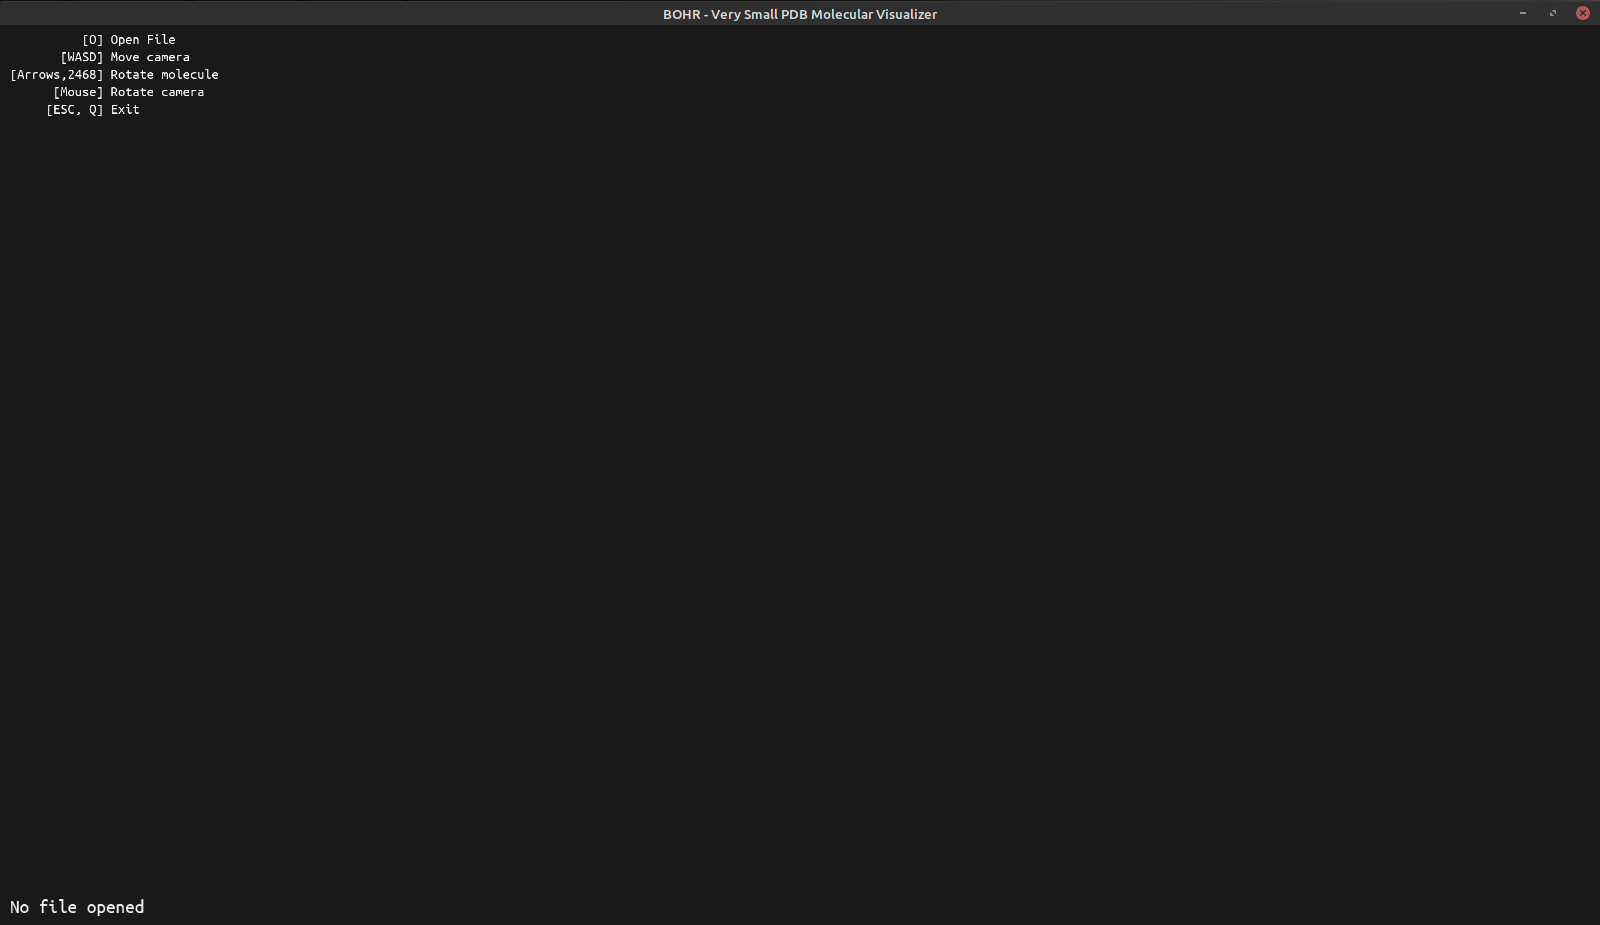
\includegraphics[width=\textwidth]{bohr-start}
    \caption[Aplicação após abertura]{Aplicação após abertura ou quando não tem uma molécula aberta para renderização.}
    \label{fig::bohr-start}
\end{figure}


\begin{figure}[!btp]
    \centering
    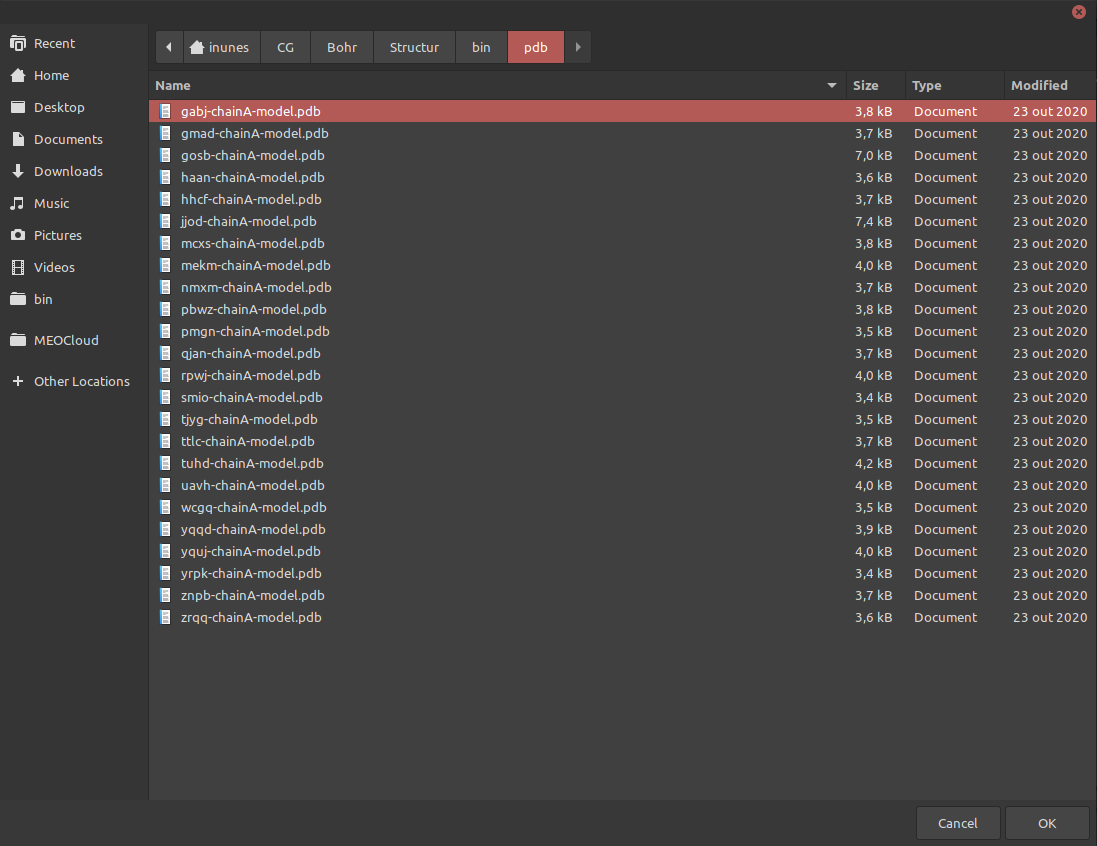
\includegraphics[width=\textwidth]{bohr-opendialog}
    \caption[Janela de diálogo para abertura de ficheiro]{Janela de diálogo do sistema operativo para abertura de um novo ficheiro \ac{PDB}.}
    \label{fig::bohr-opendialog}
\end{figure}


\begin{figure}[!btp]
    \centering
    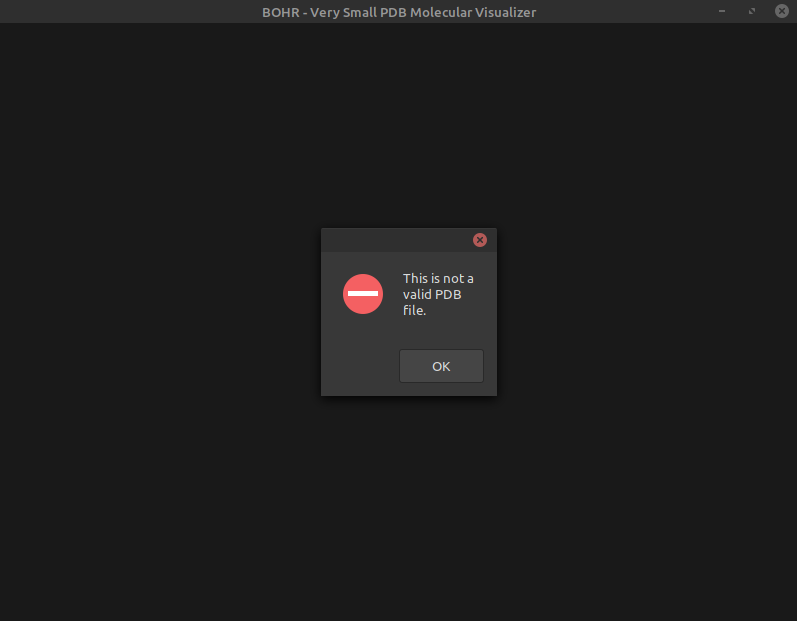
\includegraphics[scale=1.0]{bohr-error}
    \caption[Mensagem de erro]{Mensagem de erro caso o ficheiro não seja válido.}
    \label{fig::bohr-error}
\end{figure}


\begin{figure}[!btp]
    \centering
    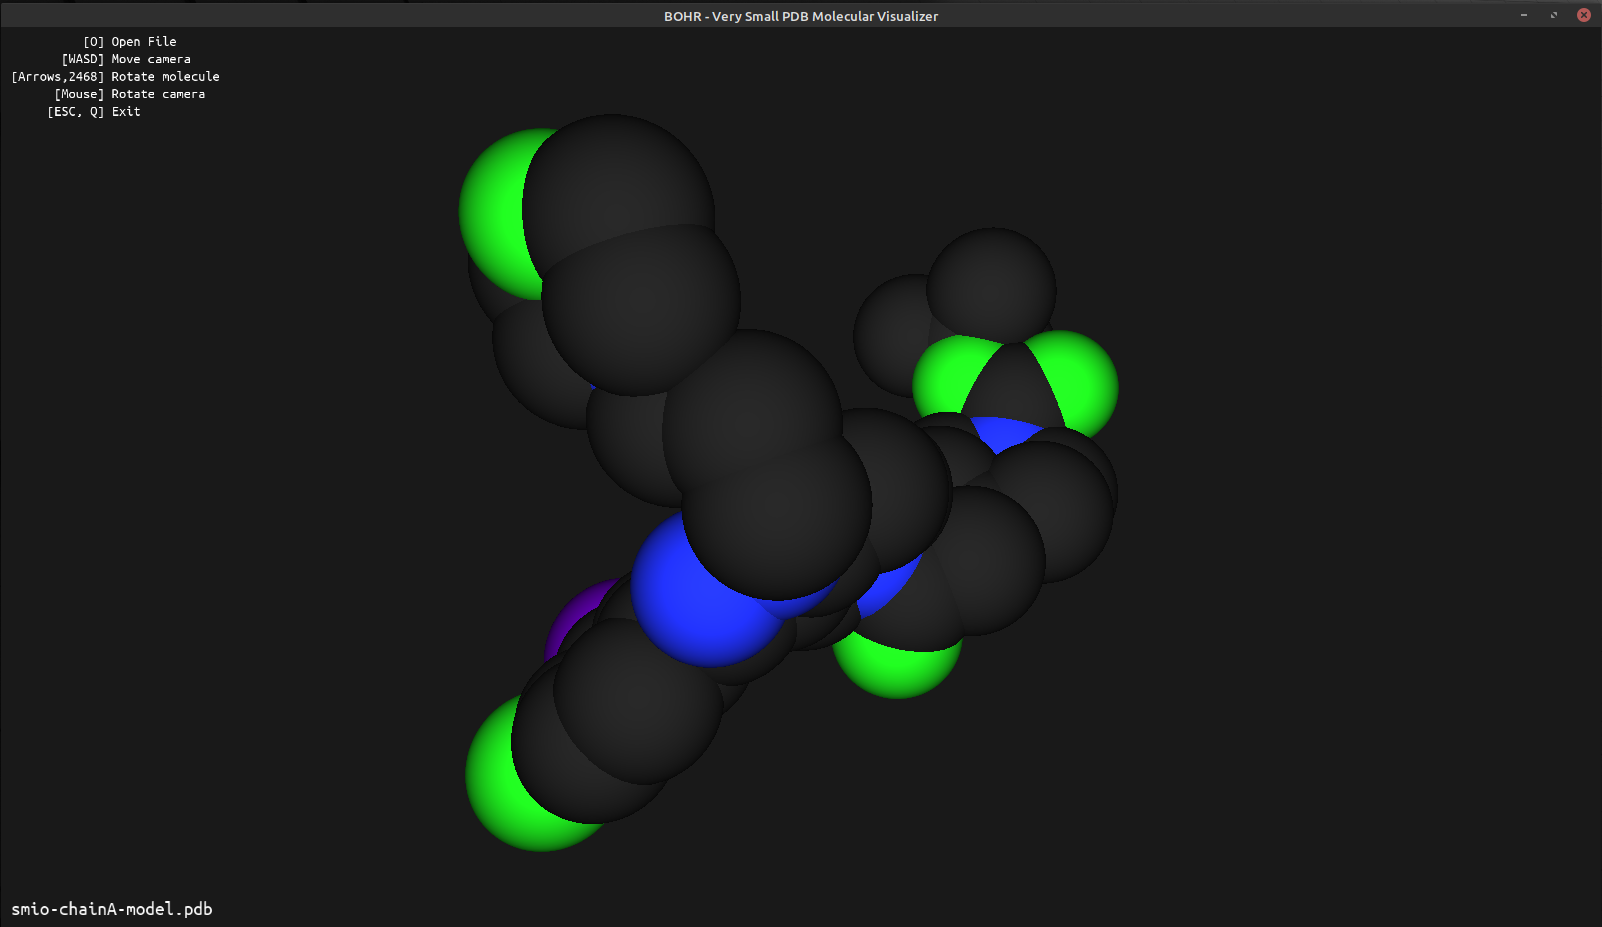
\includegraphics[width=\textwidth]{bohr-main}
    \caption[Exemplo de molécula renderizada]{Exemplo de uma molécula renderizada na aplicação após interpretação do ficheiro \ac{PDB}.}
    \label{fig::bohr-main}
\end{figure}
